% ============================================================
% Short paper — Seminario Agentes Inteligentes y LLM
% Universidad Nacional de Luján — 2026
% Formato: Springer LNCS (clase llncs)
%
% Compilar (pdfLaTeX):
%   pdflatex main  →  bibtex main  →  pdflatex main  →  pdflatex main
%
% La clase llncs y el estilo splncs04 vienen incluidos en Overleaf
% y en TeX Live (instalación full / paquete 'llncs').
%
% ============================================================

\documentclass[runningheads]{llncs}

\usepackage[utf8]{inputenc}
\usepackage[T1]{fontenc}
\usepackage[spanish,es-noshorthands]{babel}
\usepackage{graphicx}
\usepackage{xcolor}
\usepackage{booktabs}
\usepackage{float}
\usepackage{url}
\usepackage{listings}
\usepackage[hidelinks]{hyperref}

\renewcommand{\lstlistingname}{Listado}

% Dejar que los flotantes ocupen más página y evitar páginas semi-vacías
\renewcommand{\topfraction}{0.92}
\renewcommand{\bottomfraction}{0.85}
\renewcommand{\textfraction}{0.08}
\renewcommand{\floatpagefraction}{0.78}

% ----- Estilo para los bloques de transcripción de chat -----
\lstdefinestyle{chat}{
  basicstyle=\scriptsize\ttfamily,
  breaklines=true,
  breakatwhitespace=true,
  breakautoindent=false,
  breakindent=0pt,
  backgroundcolor=\color[gray]{0.95},
  frame=single,
  framerule=0.3pt,
  xleftmargin=3pt,
  xrightmargin=3pt,
  aboveskip=4pt,
  belowskip=2pt,
  columns=flexible,
  extendedchars=true,
  literate=%
    {á}{{\'a}}1 {é}{{\'e}}1 {í}{{\'i}}1 {ó}{{\'o}}1 {ú}{{\'u}}1
    {Á}{{\'A}}1 {É}{{\'E}}1 {Í}{{\'I}}1 {Ó}{{\'O}}1 {Ú}{{\'U}}1
    {ñ}{{\~n}}1 {Ñ}{{\~N}}1 {¿}{{?`}}1 {¡}{{!`}}1,
}

\begin{document}

\title{Sistema multiagente basado en LLM para el análisis contextual de
criptoactivos: clasificación de intención, ruteo entre agentes y recuperación de
datos en tiempo real}

\titlerunning{Sistema multiagente LLM para análisis de criptoactivos}

\author{Patricio Pittavino}
\authorrunning{P. Pittavino}

\institute{Universidad Nacional de Luján, Buenos Aires, Argentina\\
Seminario: Agentes Inteligentes y LLM\\
\email{pitta1881@gmail.com}}

\maketitle

% ============================================================
\begin{abstract}
El análisis de criptoactivos en tiempo real plantea dos problemas que los modelos de
lenguaje de propósito general no resuelven satisfactoriamente: la ausencia de datos de
mercado actuales en su conocimiento paramétrico, y la tendencia a evadir preguntas
directas de inversión con avisos genéricos que no orientan la decisión. Este trabajo
describe el diseño e implementación de un sistema multiagente que aborda ambos problemas.
La arquitectura combina un gateway que integra las APIs de Binance y CoinGecko, un
pipeline de agentes orquestado con LangGraph y Google Gemini, y un frontend conversacional
con autenticación OAuth. El núcleo del sistema es un grafo de estado de trece nodos que
clasifica la intención del usuario, recupera datos de mercado en tiempo real y —ante una
consulta de inversión— emite una recomendación estructurada (comprar / vender / mantener
a corto, mediano y largo plazo) en lugar de derivar la decisión hacia un asesor externo.
El sistema incorpora además memoria conversacional con seguimiento contextual y
persistencia por usuario de las conversaciones, que pueden recuperarse y continuarse en
sesiones posteriores. Los resultados muestran la viabilidad de un agente de dominio acotado
capaz de combinar razonamiento fundamentado en datos reales con capacidad de recomendar,
sin renunciar a un aviso de responsabilidad honesto.

\keywords{Sistemas multiagente \and LLM \and LangGraph \and Clasificación de
intención \and Recuperación de datos en tiempo real \and Agentes conversacionales \and
Criptoactivos}
\end{abstract}

% ============================================================
\section{Introducción}

El mercado de criptoactivos es, por naturaleza, volátil: los precios pueden desplazarse
varios puntos porcentuales en minutos y las condiciones que definen una oportunidad de
compra o venta cambian con cada bloque de transacciones. Un modelo de lenguaje entrenado
con datos históricos carece de esa información por definición; cuando se le consulta sobre
precios actuales, o bien genera cifras plausibles pero incorrectas, o bien reconoce su
limitación sin ofrecer alternativa alguna~\cite{ji2023survey}.

Hay, sin embargo, un segundo problema menos obvio pero más determinante en la práctica.
Cuando un usuario le pregunta a un asistente generalista \emph{«¿debería vender mis ETH
ahora?»}, la respuesta habitual es una combinación de advertencias legales y
recomendaciones de consultar a un asesor financiero certificado. Esa respuesta, aunque
técnicamente cauta, no ayuda a quien necesita tomar una decisión hoy con la información
que tiene disponible. Un analista de mercado humano con acceso a los mismos datos daría su
lectura: puede equivocarse, pero al menos se compromete con una postura. La pregunta que
motiva este trabajo es si un agente de dominio acotado puede hacer lo mismo, y bajo qué
condiciones.

Este trabajo presenta un sistema multiagente que adopta ese compromiso: recupera datos
reales de mercado, clasifica la intención del usuario, rutea la consulta al subgrafo
especializado correspondiente y, cuando la pregunta lo requiere, emite una recomendación
accionable fundamentada en los datos recién obtenidos. El objetivo no es reemplazar al
analista experto, sino proporcionar la señal que el usuario necesita para decidir —con un
aviso de responsabilidad honesto, pero sin esquivar la pregunta. El trabajo se desarrolló
en el marco del Seminario Agentes Inteligentes y LLM de la Universidad Nacional de Luján.

% ============================================================
\section{Estado del arte}

La arquitectura ReAct~\cite{yao2023react} estableció la base conceptual de los agentes LLM
que intercalan razonamiento con acciones sobre herramientas externas: en lugar de generar
una respuesta directa, el modelo emite pasos de razonamiento y acciones que se ejecutan en
el entorno, incorporando los resultados al contexto antes del siguiente paso. Este patrón
resuelve directamente el problema de los datos desactualizados, ya que el agente no
necesita conocer el precio de un activo si puede consultarlo en tiempo de inferencia.

LangGraph~\cite{langchain2024langgraph} extiende ese paradigma con grafos de estado
explícitos: los nodos son funciones que transforman un estado compartido y las aristas
—potencialmente condicionales— determinan el siguiente nodo en función de los valores del
estado. Esto permite definir flujos de múltiples pasos con bifurcaciones, algo esencial
cuando el análisis requiere encadenar llamadas a varias APIs y modelos según el tipo de
consulta.

El problema de las alucinaciones —generación de información plausible pero incorrecta—
está documentado extensamente~\cite{ji2023survey}. La generación aumentada por recuperación
(RAG)~\cite{lewis2020rag} y el uso de herramientas externas~\cite{schick2023toolformer} son
las respuestas dominantes: en lugar de confiar en el conocimiento paramétrico del modelo,
se lo ancla en datos recuperados en tiempo de inferencia. Este trabajo adopta ese principio
de forma estricta —ningún nodo del grafo afirma precios o fundamentales sin haberlos
obtenido de una API— y lo extiende con un mecanismo de compuerta que detiene el pipeline si
los datos no son válidos. En cuanto a la sobre-cautela de los asistentes generalistas
frente a preguntas de inversión, se trata de una restricción deliberada de política de uso;
un agente de dominio acotado, con acceso verificable a datos actuales y un alcance declarado
explícitamente, puede operar bajo un contrato distinto con el usuario.

% ============================================================
\section{Metodología y arquitectura}

\subsection{Arquitectura general del sistema}

El sistema se organiza en tres servicios independientes que se comunican por HTTP
(Figura~\ref{fig:arquitectura}). El \emph{frontend}, implementado con React y Vite,
gestiona la interfaz conversacional, los widgets de mercado (mapa de calor, gráfico de
velas, banner de precios) y la autenticación OAuth con Google a través de Supabase. El
\emph{gateway}, desarrollado con Fastify y TypeScript, concentra la integración con las
fuentes de datos externas (Binance para precios y velas, CoinGecko para datos
fundamentales) y actúa como proxy hacia el servicio de agentes. El \emph{servicio de
agentes}, implementado con FastAPI, expone un único endpoint (\texttt{POST /run-agent})
que recibe el mensaje del usuario, el historial compacto y metadatos de sesión, ejecuta el
grafo LangGraph y devuelve el estado resultante.

La separación de responsabilidades tiene un propósito preciso: el gateway es el único
punto de contacto con las APIs de mercado para los widgets síncronos, mientras que el
servicio de agentes accede a esas mismas fuentes dentro del grafo cuando el análisis lo
requiere, sin acoplar ambos contextos de uso.

Esta división tiene además una consecuencia organizativa. Como cada servicio encapsula una
responsabilidad acotada y el único acoplamiento entre ellos es el contrato HTTP/JSON que
intercambian, cada uno puede evolucionar, probarse y desplegarse por separado mientras ese
contrato se respete. Esto acota el alcance de cada cambio y habilita que distintas personas
o equipos trabajen en paralelo sobre cada servicio —mejorar el pipeline del agente,
rediseñar el frontend o cambiar una API externa sin afectar a los demás— en lugar de
coordinar todo sobre una única base de código monolítica.

\begin{figure}[tbp]
\centering
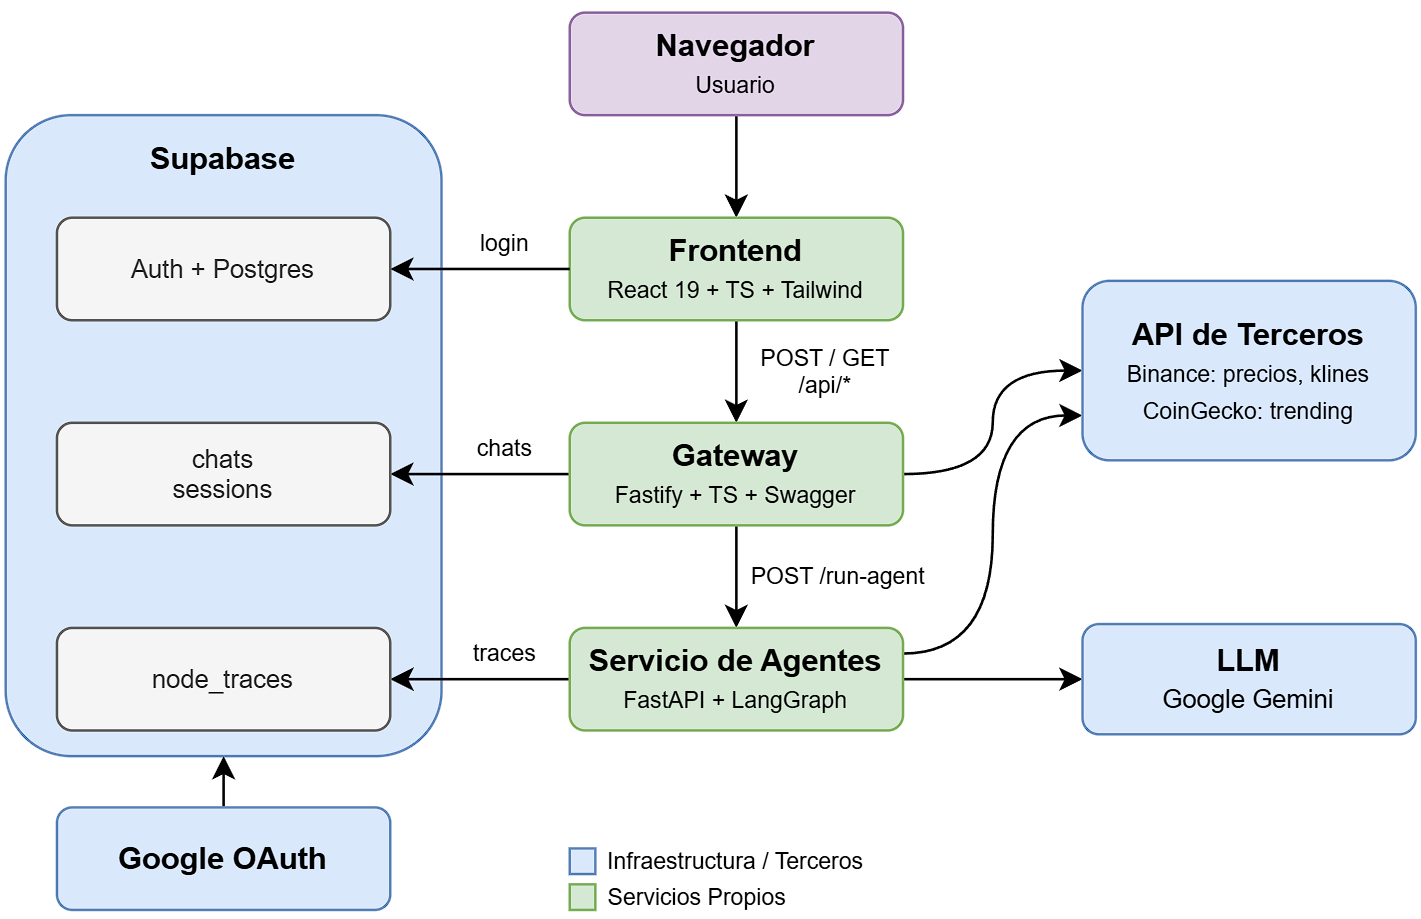
\includegraphics[width=\textwidth]{imagenes/arquitectura.png}
\caption{Arquitectura general del sistema en tres servicios (frontend, gateway y servicio
  de agentes) y sus integraciones con las APIs externas y con Supabase.}
\label{fig:arquitectura}
\end{figure}

\subsection{Pipeline multiagente}

El núcleo del sistema es un \texttt{StateGraph} de LangGraph con trece nodos conectados
mediante aristas condicionales (Figura~\ref{fig:grafo}). El estado compartido
(\texttt{ChatState}) acumula el mensaje original, el historial conversacional, los datos
recuperados de las APIs, los análisis parciales de cada nodo especialista y, finalmente, la
respuesta de síntesis.

\begin{figure}[tbp]
  \centering
  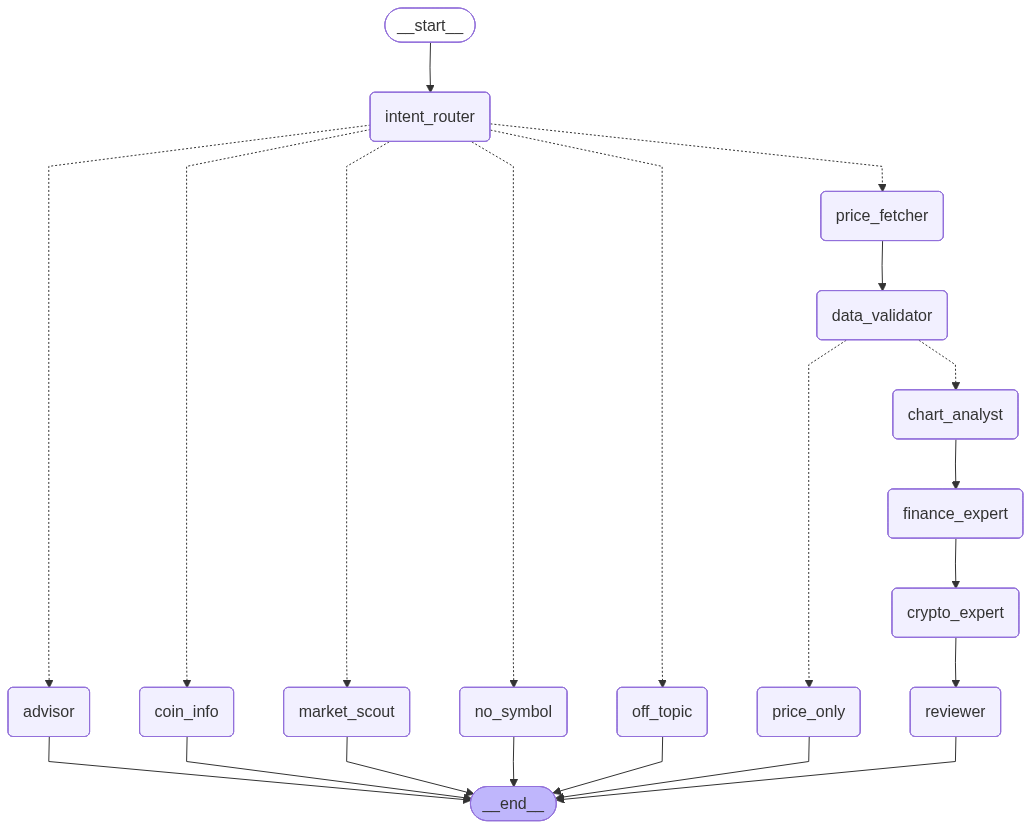
\includegraphics[width=0.62\textwidth]{imagenes/graph.png}
  \caption{Grafo de estados del pipeline multiagente, generado automáticamente por
    LangGraph al iniciar el servicio. Cada nodo es una función asíncrona que transforma el
    estado compartido; las aristas condicionales se evalúan en tiempo de ejecución.}
  \label{fig:grafo}
\end{figure}

\noindent\textbf{Clasificación de intención.} El nodo inicial, \texttt{intent\_router},
realiza una llamada al LLM con el mensaje del usuario y el historial reciente para
clasificar la consulta en uno de siete intents: \emph{market\_overview},
\emph{recommendation}, \emph{analysis}, \emph{price\_only}, \emph{coin\_info},
\emph{no\_symbol} u \emph{off\_topic}. La clasificación determina el nodo siguiente. No se
trata de coincidencia de patrones sobre el texto, sino de razonamiento sobre la intención:
la misma pregunta «¿cómo está el BTC?» puede clasificarse como \emph{price\_only} o como
\emph{analysis} según el contexto conversacional previo.

\noindent\textbf{Ruteo condicional.} El intent \emph{recommendation} activa
\texttt{advisor}, que descarga los tickers de Binance, construye dos universos de activos
—uno conservador con símbolos curados y otro amplio con los pares de mayor volumen— e
infiere el perfil de riesgo del usuario a partir del texto de la consulta, devolviendo una
cartera diversificada ajustada a ese perfil. Para los intents de análisis de un activo
específico, el grafo pasa por \texttt{price\_fetcher} (precio actual y velas de siete días
en Binance) y luego por \texttt{data\_validator}, que actúa como compuerta: si los datos
son inválidos o están ausentes, el flujo deriva a \texttt{price\_only}, que responde
honestamente que no hay datos disponibles; si son válidos, se activa la cadena completa
\texttt{chart\_analyst} $\rightarrow$ \texttt{finance\_expert} $\rightarrow$
\texttt{crypto\_expert} $\rightarrow$ \texttt{reviewer}.

\noindent\textbf{Síntesis y el problema de la evasión.} Los tres nodos especialistas
producen análisis independientes desde sus perspectivas (técnica, fundamental y de
ecosistema). El nodo \texttt{reviewer} los sintetiza y emite el veredicto estructurado:
una recomendación de \textsc{comprar}, \textsc{vender} o \textsc{mantener} para los
horizontes de corto, mediano y largo plazo, seguida de un análisis y un aviso de
responsabilidad. Este es el punto donde el sistema adopta una postura distinta a la de los
asistentes generalistas: en lugar de derivar la decisión, se compromete con una
recomendación basada en los datos que acaba de recuperar. No es una certeza; es la señal
que el usuario necesita para decidir.

\noindent\textbf{Grounding y memoria conversacional.} Todo nodo que afirma algo sobre el
mercado lo hace a partir de datos recuperados en la misma invocación; ninguno confía en el
conocimiento paramétrico del modelo para cifras de precio, capitalización o volumen. El
nodo \texttt{coin\_info} resuelve el identificador del activo en CoinGecko exigiendo
coincidencia exacta del símbolo: una política más restrictiva que tomar el primer resultado
por ranking, pero que evita confundir activos (buscar el ticker \texttt{RE} devolvería
Ethereum como primer resultado porque ninguna moneda usa ese símbolo y ETH encabeza por
capitalización). Durante una conversación, el historial vive en el cliente, que envía un
resumen compacto de hasta diez turnos en cada consulta; el \texttt{intent\_router} lo usa
para resolver referencias implícitas («¿debería vender?» tras un análisis hereda el símbolo
anterior) sin arrastrar contexto cuando la nueva pregunta es ajena al dominio. Cada turno se
persiste además por usuario en Supabase, de modo que las conversaciones anteriores pueden
listarse y recuperarse para continuarlas en una sesión posterior.

\subsection{Empaquetado y despliegue continuo}

Cada servicio se empaqueta en su propia imagen de contenedor. El gateway usa una
construcción \emph{multi-stage} que compila el frontend y lo sirve junto a la API desde un
único origen, lo que elimina la configuración de CORS y de URLs absolutas en producción; el
servicio de agentes se distribuye como una imagen de Python independiente. Sobre ese
empaquetado se monta un flujo de integración y despliegue continuos: en cada \emph{push} a
la rama principal, un \emph{workflow} de GitHub Actions verifica tipos y construye el
frontend como compuerta de calidad, y la plataforma de despliegue (Railway) reconstruye las
imágenes a partir de los \emph{Dockerfiles} y publica la nueva versión sin pasos manuales.
Combinado con la independencia entre servicios, esto permite desplegar cada uno por separado
y reduce la deriva de configuración entre desarrollo y producción.

% ============================================================
\section{Resultados y evidencias de funcionamiento}

\subsection{El diferenciador: respuesta accionable frente a evasión}

El escenario que mejor ilustra la propuesta es la pregunta directa de inversión. Ante la
misma consulta, el comportamiento difiere de forma significativa entre un asistente
generalista y este sistema (Listado~\ref{lst:contraste}).

\begin{lstlisting}[style=chat, float=htbp, label={lst:contraste}, caption={Misma consulta «¿debería vender mis ETH?»: el LLM generalista evade; el sistema se compromete con un veredicto accionable.}]
Usuario: ¿Debería vender mis ETH ahora?

LLM generalista:
No puedo proporcionar asesoramiento financiero personalizado.
Las inversiones en criptoactivos conllevan riesgos significativos
y altamente especulativos. Te recomiendo consultar a un asesor
financiero certificado antes de tomar cualquier decisión.
-------------------------------------------------------------
Sistema (este trabajo):
 Mirá, ETH está en una situación bastante complicada porque cotiza a $1,615.29 tras una caída del 2.96% en las últimas 24 horas, lo que confirma que la presión vendedora sigue mandando. La estructura técnica es netamente bajista y el activo se encuentra operando peligrosamente cerca de su mínimo semanal, sin señales claras de que la tendencia vaya a revertirse pronto.
  - Recomendacion
     Corto plazo:   VENDER
     Mediano plazo: VENDER
     Largo plazo:   MANTENER
  - Analisis
  La estructura de ETHUSDT es claramente bajista, con una presión vendedora dominante que ha llevado al precio a operar cerca de su mínimo diario de $1,552.95. El volumen de 352,751 unidades confirma que los vendedores mantienen el control total y no muestran signos de agotamiento, lo que descarta cualquier intento de reversión a corto plazo. Técnicamente, el activo se encuentra en una posición vulnerable, ya que cualquier rebote encontrará una resistencia pesada en los $1,779.90, nivel que actúa como techo del rango reciente. La volatilidad se mantiene alta, con un rango de 140 dólares en las últimas 24 horas, lo que vuelve muy arriesgado mantener posiciones largas en este contexto. El soporte crítico de los $1,552.95 es el único nivel que separa al activo de una profundización del desplome actual. En resumen, la relación riesgo-beneficio es desfavorable para los compradores, y la falta de soporte sólido sugiere que la tendencia negativa podría extenderse si se pierde el mínimo semanal.
\end{lstlisting}

La diferencia no radica en la calidad del análisis —que puede ser mayor en un servicio
especializado de trading— sino en la disposición a comprometerse con una respuesta dentro
del dominio para el que el sistema fue diseñado. La señal, incluso si no es perfecta, tiene
más valor para el usuario que la no-respuesta. La Figura~\ref{fig:chat} muestra esa
respuesta integrada en la interfaz, junto a los widgets de mercado en tiempo real que
acompañan la conversación.

\begin{figure}[tbp]
  \centering
  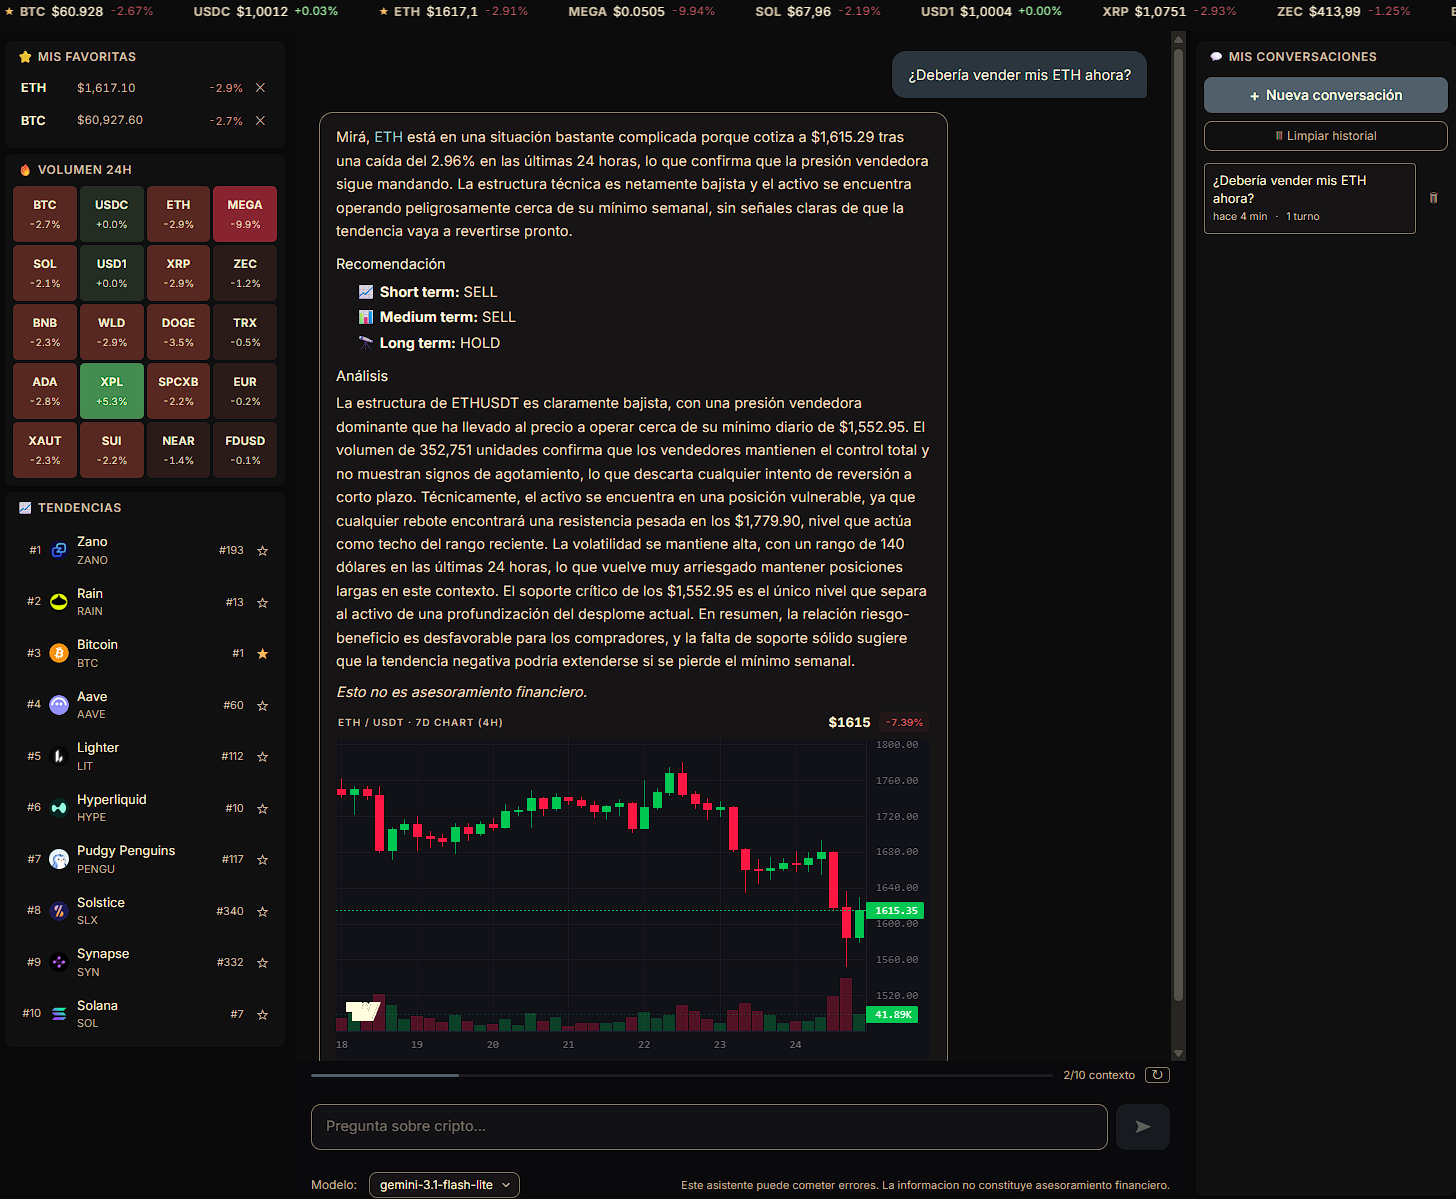
\includegraphics[width=\textwidth]{imagenes/chat-recomendacion.png}
  \caption{Panel principal: widgets de mercado en tiempo real (izq.) y chat con una
    recomendación estructurada (der.).}
  \label{fig:chat}
\end{figure}

\subsection{Escenarios evaluados}

Durante el desarrollo se evaluaron, además del caso anterior, los siguientes escenarios:
consulta de precio simple (activación de \texttt{price\_only} con datos en tiempo real),
análisis multinodo de un activo con datos válidos (cadena completa de cuatro especialistas
más \texttt{reviewer}), memoria conversacional (carryover correcto del símbolo sin
mencionarlo de nuevo), preguntas fuera de dominio (redirección amable sin reproducir el
análisis previo) y activos inexistentes (respuesta honesta sin inventar cifras). En todos
los casos el comportamiento observado coincidió con el ruteo esperado del grafo, lo que
respalda la robustez de la clasificación de intención como mecanismo de control del flujo.

% ============================================================
\section{Conclusiones y líneas futuras}

Este trabajo presentó un sistema multiagente para análisis de criptoactivos cuyas
contribuciones se articulan en tres ejes. El primero es el \emph{grounding} sistemático
contra la alucinación: ningún nodo afirma datos de mercado sin haberlos recuperado en
tiempo de inferencia, y el nodo \texttt{data\_validator} detiene el pipeline cuando esos
datos no son válidos. El segundo es la clasificación de intención como mecanismo de ruteo,
que permite especializar cada nodo en una tarea precisa; la distinción entre
\emph{off\_topic} y \emph{no\_symbol} —colapsada en una sola categoría en una primera
implementación— resultó determinante para que la memoria conversacional funcionara. El
tercero, y el más relevante desde la perspectiva del usuario, es comprometerse con una
recomendación en lugar de evadir la pregunta: un sistema de dominio acotado, con acceso
verificable a datos actuales, puede adoptar un contrato distinto al de los asistentes
generalistas, asumiendo la incomodidad de recomendar con un aviso de responsabilidad
honesto.

Entre las limitaciones, la más importante es que las recomendaciones no fueron validadas
retrospectivamente contra movimientos reales de mercado: el sistema produce señales
razonadas, no señales evaluadas. Tampoco pretende sustituir a un analista experto, y depende
de APIs públicas cuyos límites de tasa pueden afectar la disponibilidad de los datos en
escenarios de alta concurrencia. Otra limitación es que el acceso al agente está acoplado a
una sesión interactiva: el endpoint de chat exige un token que hoy solo se obtiene mediante
el inicio de sesión con Google en el navegador, de modo que un cliente programático no puede
consumirlo (los endpoints de mercado, en cambio, son públicos). Las líneas de trabajo futuro
más significativas son: incorporar recuperación aumentada sobre noticias y reportes recientes
(RAG)~\cite{lewis2020rag} para enriquecer el análisis fundamental; personalizar tanto el
dashboard como el agente en función del historial de conversaciones del usuario —las
criptomonedas que consulta con frecuencia y el perfil de inversor que se infiere de sus
interacciones—, adaptando las vistas y el sesgo de las recomendaciones a sus intereses;
habilitar un acceso no interactivo a la API mediante el inicio de sesión anónimo de Supabase
(que emite un token válido sin credenciales y conserva un identificador por usuario), junto
con límites de tasa, de modo que el sistema pueda integrarse de forma \emph{headless} sin
perder la traza de auditoría; y diseñar un conjunto de evaluación que mida la calidad de las
recomendaciones frente a evoluciones reales del mercado, cerrando el ciclo entre la señal que
emite el agente y su utilidad práctica.

% ============================================================
\bibliographystyle{splncs04}
\bibliography{referencias}

\end{document}
